%!TEX root = main.tex
\section{Deep outdoor Photometric Stereo network}
\label{sec:proposed_method}

This section presents our CNN-based approach designed to address ambiguities that arise in single-day outdoor PS reconstruction. It does so by using deep learning to model prior knowledge on object geometry, material properties, as well as their local spatial correlation and interaction with natural sky light. In order to build such knowledge base, one needs a large number of images depicting various objects lit by outdoor lighting throughout the day, over different geographic locations and days over the year; finally, the surface normal map of each object is also required. Unfortunately, no such large-scale dataset currently exists, so a natural choice is to synthesize realistic data to train our network. We begin by presenting our problem formulation, CNN architecture, followed training procedure and data generation.

\subsection{Image formation model} % includes illumination subspace (analemmata)

% sky model can represent sun position, turbidity, etc... but not clouds, that's why we assume clear skies

% BRDF can be any family, we chose isotropic GGX which is popular these days...

Consider an image pixel that depicts a small area of an object's surface, with a normal vector ${\bf n} \in \Reals^3$ and material reflectance described by a bidirectional reflectance distribution function (BRDF) $\rho(\cdot)$. When viewed from direction \mbox{${\bf v} \in \Reals^3$}, the RGB color ${\bf b}_t \in \Reals^3$ of this pixel at daytime $t$ is modeled as
%
\begin{equation}
{\bf b}_t = \int_{\Omega_{\bf n}} \rho(\boldomega, {\bf v}, {\bf n}) {\bf  L}_t(\mathbf{\boldomega}) (\boldomega^T{\bf n}) V(\boldomega) d\omega \,,
\label{eq:ifm_singlepixel}
\end{equation}
%
where $\boldomega$ is a direction of incoming light within the hemispherical domain $\Omega_{\bf n}$, ${\bf L}_t(\mathbf{\boldomega})$ is the RGB intensities (color) of the incoming light at time $t$, and $V(\boldomega)$ is a binary visibility encoding self-shadowing. Here $t$ denotes the {\em actual solar time} at the target object location.

Our goal is to invert the above rendering equation and recover the surface normal ${\bf n}$ based on the observed changes in pixel intensities ${\bf b}_t$, which are caused by the changing natural illumination ${\bf L}_t(\mathbf{\boldomega})$ as $t$ varies throughout the day. However, as discussed above, a solution based solely on the photometric cue is rarely uniquely defined and stable in outdoor PS due to the limited motion of the sun, leading to insufficient variability in ${\bf L}_t(\mathbf{\boldomega})$ and, thus, ${\bf b}_t$~\cite{holdgeoffroy-3dv-15}.

Therefore, instead of considering a single pixel $\mathbf{b}_t$, we reformulate our goal and instead aggregate additional RGB image data within a \emph{neighborhood} ${\bf B}_t \in \Reals^{16 \times 16 \times 3}$, depicting a larger surface patch centered at the pixel $\mathbf{b}_t$. Now we seek to learn a predictor ${\bf N} = f({\bf B}_{t_1}, \ldots, {\bf B}_{t_T})$, where $T$ denotes the number of input images and ${\bf N} \in \Reals^{16\times 16\times 3}$ has the patch normals. In this paper, $T=8$ but we experiment with other values in sec.~\ref{sec:ablation_study}. This approach is motivated by the fact that complex object geometry is often made up of simpler, small surface patches presenting highly correlated surface normals and material properties. A natural way to obtain this predictor $f(\cdot)$ is to train a CNN that learns a nonlinear function of local surface features that are highly correlated with the normal ${\bf n}$ at the center of the patch. We train our network on a large synthetic database of surface patches realistically rendered with a standard GGX shader for $\rho(\cdot)$, with varying diffuse and specular parameters, and using the Ho\v{s}ek-Wilkie physically-based sky model~\cite{hosek-tog-12} for the spherical function ${\bf L}_t(\mathbf{\boldomega})$, as described next.

%\eqref{eq:ifm_singlepixel} is non-linear due to the reflectance function, and  and approximating the 2-source PS problem. Both issues can solved by learning priors that extend the photometric constraints.

% ambiguity, normals are locally correlated within a patch
% semi-calibrate, we don't require a light probe...
% assumptions... then architecture

% clouds, as long as don't obscure sun, change predominant direction of illumination considerably far from analemmata subsbace in Fig, should be ok. See experiments for sensitivity analysis.


\subsection{Illumination model: the solar analemma}
\label{sec:analemma}

We follow a semi-calibrated PS approach that does not require known lighting environments~\cite{yu-iccp-13} nor complete camera geolocation data~\cite{jung-cvpr-15}. Our method only assumes that: (1) the object images are captured at roughly predefined times of the day, $t \in \{t_1, t_2, \ldots, t_T \}$; (2) the sun is unobstructed by clouds at these times; and (3) the camera is orthographic and faces approximately North (or South). We later (sec.~\ref{sec:analysis}) analyze the robustness of our network with respect to departures from these ideal conditions and discuss how assumption~(3) can be relaxed.

Together, these assumptions constrain the sun position to lie within an ``8-figure'' subspace at each time $t$, known as a solar {\em analemma}, whose shape also varies with geographical location (fig.~\ref{fig:solar-analemma}). For a given time $t$, the sun may be positioned at different locations depending upon the selected date and latitude, as prescribed by the analemma. The neural network is thus expected to adapt to this (constrained) variability in sun position and associated intensity. As shown in fig.~\ref{fig:solar-analemma}-(a,b), for a given timestamp and latitude, the sun position spans relatively small angular ranges, which still remain quite constrained even when considering geographical locations sampled over the Northern Hemisphere (fig.~\ref{fig:solar-analemma}-(c)) (note that a similar plot would be obtained by sampling the Southern Hemisphere with the camera facing south). 

% On sunny days, illumination can change greatly depending on the geographical location of the observer and the date. On rare occasions, it can even provide sufficient contraints for photometric stereo~\cite{shen-pg-14}.

% One of the most notable effect is the solar analemma, namely the path of the sun in the sky throughout the year as viewed at a fixed time of day. Some analemmata like the ones shown in fig.~\ref{fig:sun_positions} exhibit over 45 degrees of azimuthal range through the year, especially early morning and late afternoon. This effect is different on the zenithal angle, where a variation similar in amplitude can be witnessed around noon. As the sun is the dominant light source on a sunny day, modeling this pattern can give hints to reason on the observed scene.

% This variability of the world over the course of a day is not accurately captured by currently available outdoor photometric stereo datasets. 

\begin{figure}[t]
    \centering
    \begin{tabular}{c@{\extracolsep{\fill}}cc}
        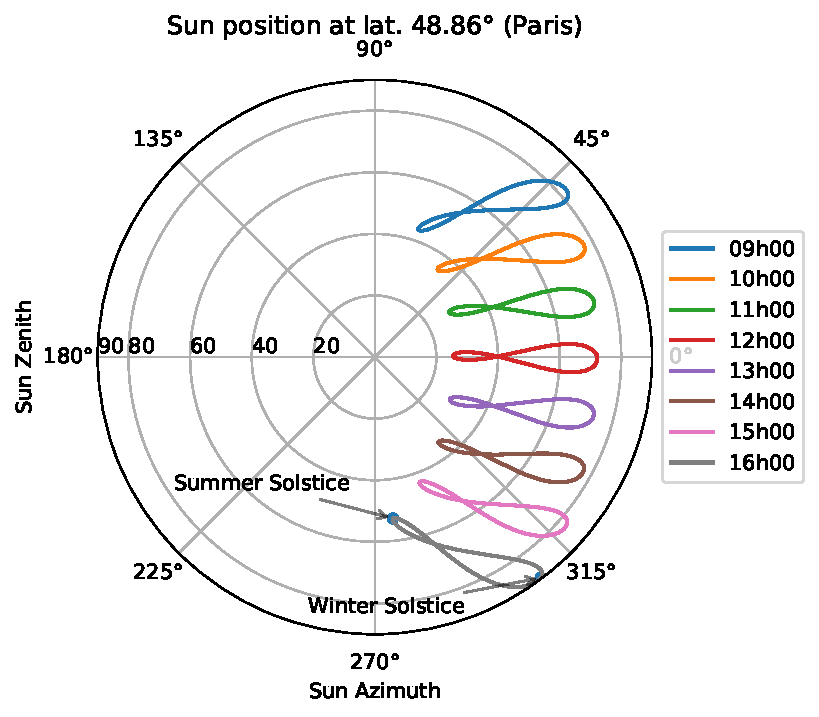
\includegraphics[width=0.34\linewidth]{figures/sun_pos/sunpos_paris.pdf} &
        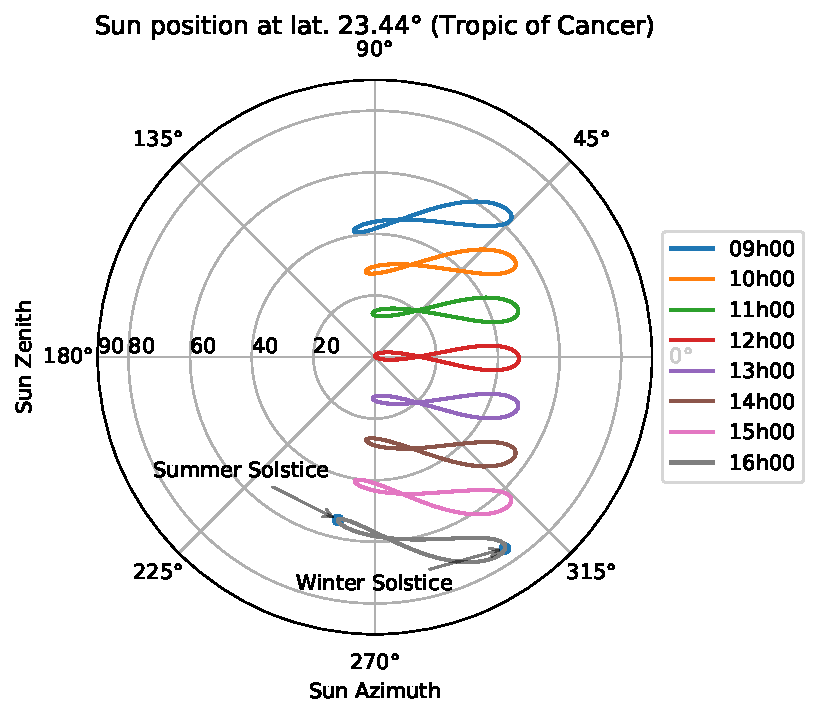
\includegraphics[width=0.34\linewidth]{figures/sun_pos/sunpos_nt.pdf} &
        \makecell[t]{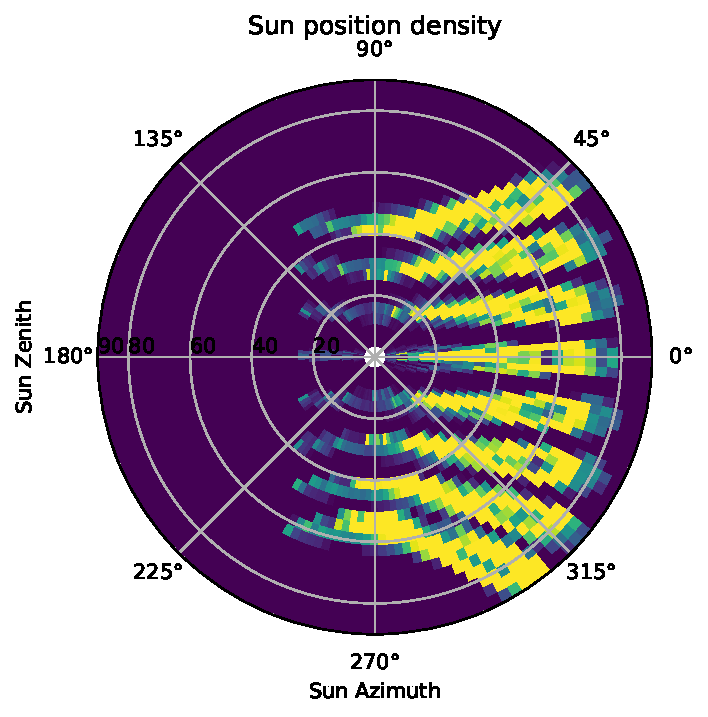
\includegraphics[width=0.29\linewidth]{figures/sun_pos/sunpos_all.pdf} \vspace{-5pt}\\
        \hspace{3pt}
\includegraphics[width=0.22\linewidth]{figures/sun_pos/colorbar_sunpos_prob_horizontal.pdf}} \\
        \hspace{-11pt}(a) & \hspace{-11pt}(b) & \hspace{3pt}(c)
    \end{tabular} \\
    \caption{Solar analemma: position of the sun in the sky at a specific time of the day and throughout a year over (a) Paris and (b) the Tropic of Cancer. Note how the analemmas spread over a wide range of zenith and azimuth angles over the course of a year. (c)~Probability of the sun location in the sky for our training set.}
    \label{fig:solar-analemma}
\end{figure}

% Solar analemma: position of the Sun in the sky over the course of a year, as viewed at a fixed time of day and from a fixed location on the Earth

The physically-based parametric sky model of Ho\v{s}ek and Wilkie~\cite{hosek-tog-12} is used to obtain the spherical illumination function ${\bf L}_t(\mathbf{\boldomega})$ in eq.~\eqref{eq:ifm_singlepixel}. The model represents the spectral sky radiance as a parametric function of the sun position, sky turbidity and ground albedo. Here, turbidity is set to 2, which corresponds to a clear day, and ground albedo to 0.3. Note that we do not model light scattering caused by clouds obscuring the sun and thus assume the sun is fully visible in the sky.

\subsection{Network architecture}
\label{sec:architecture}

We now turn to the design of the function ${\bf N} = f({\bf B}_{t_1}, \ldots, {\bf B}_{t_T})$ introduced above, which is done through a Convolutional Neural Network (CNN). An overview of its proposed architecture is shown in fig.~\ref{fig:architecture}. The network takes $T=8$ input $16 \times 16$ image patches, extracted from 8 images captured at regular intervals $\Delta t$ between 9:00 and 16:00 solar time throughout a single sunny day. The first layer is composed of 32 channels of $5 \times 5$ filters with shared weights across the 8 inputs. The resulting feature maps are subsequently concatenated in a single $14 \times 14 \times 256$ feature tensor. A second convolutional layer is then used, yielding 256 channels, followed by 3 residual blocks as defined in the resnet-18 architecture~\cite{he-cvpr-16}. Lastly, 2 fully-connected layers (FC) are used to produce a $16 \times 16 \times 3$ patch of estimated normals $\mathbf{n}$. Note that we experimented with fully-convolutional architectures~\cite{taniai-arxiv-18} but found the FC layers to yield better results. The ELU activation function~\cite{clevert-iclr-16} is used at every convolutional and fully connected layer, except the output layer where a $\tanh(\cdot)$ function is used. Batch normalization~\cite{ioffe-icml-15} is applied at every layer except the first one and the output layer, where it could otherwise break low-level feature detectors and output distributions.

% The architecture mix of standard feed-forward convolutional and residual layers to learn the relationship between surface normals and photometric cues exhibited throughout a single day. 
% One particularity of our architecture is the large quantity of input heads of our CNN. 

\begin{figure}[t]
	\centering
	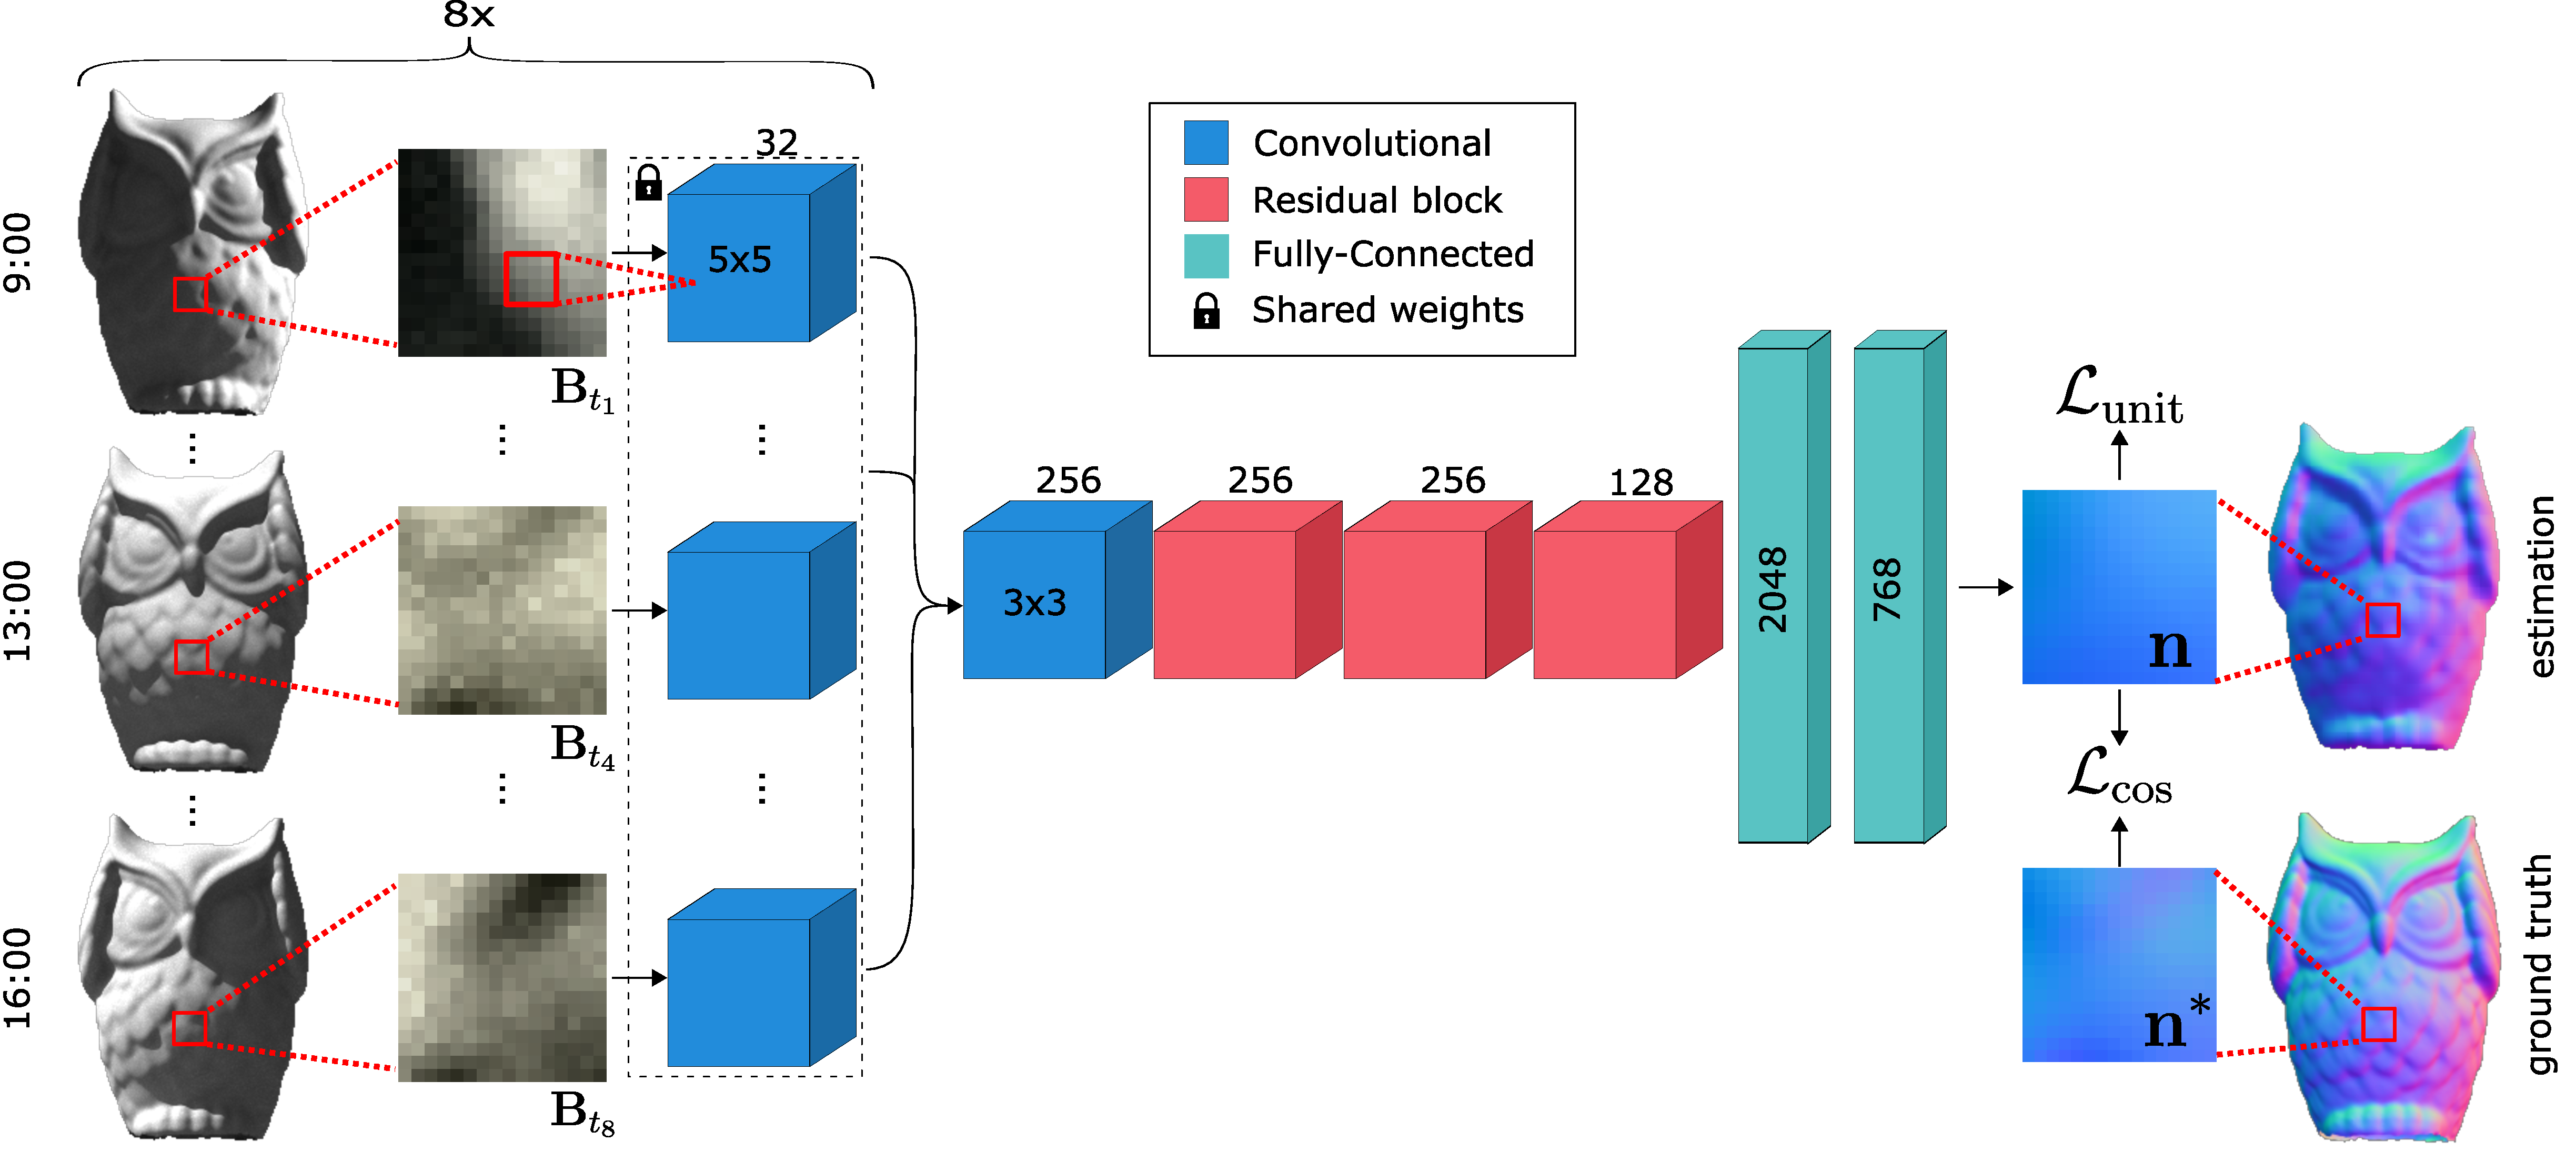
\includegraphics[width=0.8\linewidth]{figures/architecture.pdf}
	\caption[]{Our novel CNN architecture for deep single-day outdoor PS on sunny days. The network operates on $16 \times 16$ patches $\mathbf{B}_t$ of the input image, captured at 8 time intervals $t$ regularly spaced throughout a single day. The network uses convolutional (blue) and residual (red) layers before estimating the normals using fully-connected layers (green). Two losses are used to train our method, one based on the cosine distance with the ground truth $\mathbf{\hat{n}}$ and another to constrain the norm of the output vector.}
	\label{fig:architecture}
\end{figure}

%, when photometric cues alone do not yield enough information for stable reconstruction. Using 8 input images captured at predefined times $t$ at regular intervals throughout a single sunny day, our convolutional architecture provides state-of-the-art results. We make two key observations: 1) spatial priors should be learned to overcome the weak conditioning induced by the single-day constraint, 2) to help generalization to new objects and limit the size of the training set, those spatial priors should be \emph{local}. 

The $16 \times 16$ estimated normals are represented by cartesian $(x,y,z)$ components of the surface normal of the input patch. We experimented with both cartesian $(x,y,z)$ and spherical coordinates $(\theta,\phi)$ parameterization, but found the cartesian parameterization to be more stable despite its additional degree of freedom. We hypothesize this may be due to the ``wrap-around'' issue with the azimuth angle $\phi$. 

To process entire images, we crop overlapping tiles from the image with a stride of 8 pixels. Since a pixel can belong to up to 4 patches, the network produces several estimates $\mathbf{\hat{n}}$ that are then merged together using a weighted average. We use a Gaussian kernel with $\sigma=4$ centered on the middle of the patch as weighting function to perform the linear interpolation across overlapping patches. %This weighted average is used as a normal estimation confidence, where we believe the normals estimated in the center of the patch to be of higher chance of being right as the CNN sees more context around them.

\subsection{Training}

The network learns a function that estimates the patch normals $\mathbf{N}$. We define the loss to be minimized between the estimated and ground truth patch normals $\mathbf{N}$ and $\mathbf{N}^*$ respectively as the sum of two separate loss functions defined on individual patch normals $\mathbf{n}_i$, $i \in \{1, ..., N\}$ where $N = 16 \times 16 = 256$. The total loss is the sum over all $N$ individual normals: 
%
\begin{equation}
\mathcal{L}(\mathbf{N}, \mathbf{N}^*) = \sum_{i=1}^{N} \left(\mathcal{L}_{\cos}(\mathbf{n}_i, \mathbf{n}^*_i) + \mathcal{L}_{\mathrm{unit}}(\mathbf{n}_i) \right)\,.
\label{eqn:loss}
\end{equation}
%
The first term is the cosine distance between the estimated $\mathbf{n}_i$ and ground truth normal $\mathbf{n}^*_i$:
%
\begin{equation}
\mathcal{L}_{\cos}(\mathbf{n}_i, \mathbf{n}^*_i) = 1 - \frac{ \left\langle \mathbf{n}_i , \mathbf{n}^*_i \right\rangle }{ \lVert \mathbf{n}_i \rVert \lVert \mathbf{n}^*_i \rVert } \,,
\end{equation}
%
where $\left\langle \cdot , \cdot \right\rangle$ denotes the dot product. The second term enforces the unit-length constraint on the recovered normal: 
%
\begin{equation}
\mathcal{L}_{\mathrm{unit}}(\mathbf{n}_i) = \left| \; \lVert \mathbf{n}_i \rVert - 1 \; \right| \,.
\end{equation}
%
The loss in eq.~\eqref{eqn:loss} is minimized via stochastic gradient descent using the Adam optimizer~\cite{kingma-iclr-15} with an initial learning rage of $\eta = 0.001$, a weight decay $\lambda = 1\times10^{-4}$ and the recommended values $\beta_1 = 0.9$ and $\beta_2 = 0.999$. Mini-batches of 128 samples were used during training and regularized via early stopping. Training typically converges in around 250 epochs on our dataset, which is described next.



% \begin{wrapfigure}{RLH}{0.5\textwidth}
% \vspace{-2em}
% \centering
% 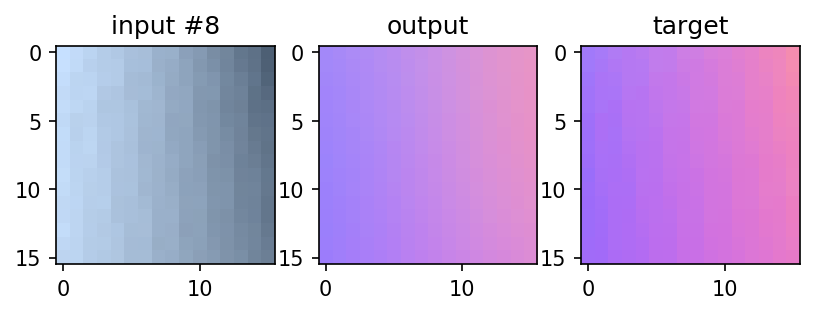
\includegraphics[width=\linewidth]{figures/training_step.png}
% \caption{Example of a validation step: 8th input (left), estimated normals $\mathbf{\hat{n}}$ (center) and ground truth normals $\mathbf{n}$ (right).}
% \label{fig:training_step}
% \vspace{-2em}
% \end{wrapfigure}


\subsection{Training dataset}
\label{sec:training_dataset}

To train our predictor function $f(\cdot)$, we rely on a large training dataset of synthetic objects, lit by a physically-based outdoor daylight model. To generate a single 8-images set of inputs, we randomly select a combination of: 1) object shape, 2) material properties, and 3) geo-temporal coordinates for lighting conditions. We now detail how each of these 3 choices are made. 

% Shape
Since the neural network only sees patches of $16 \times 16$ pixels, its receptive field is, by design, not large enough to learn priors on whole object shapes. Therefore, our dataset contains a wide variety of local surface curves. We used the blob dataset from~\cite{johnson-cvpr-11} as training models. We also added simple  primitives (cube, sphere, icosahedron, cone) to the dataset. A validation set, comprised of one of the blobs models that was kept from the training set as well as some models from the Stanford 3D Scanning Repository~\cite{curless-cg-96} and the owl model used in~\cite{holdgeoffroy-iccp-15}, was also created. All blobs and geometric primitives are randomly rotated about their centroid. 

% Materials

To model a wide range of surface appearance ranging from diffuse to glossy, we employ a linear combination of a lambertian and a microfacet model: 
%
\begin{equation}
\rho(\boldomega, {\bf v}, {\bf n}) = \boldrho_c (\alpha + (1-\alpha)\rho_\text{GGX}(\boldomega, {\bf v}, {\bf n}, \sigma)) \,,
\label{eq:brdf}
\end{equation}
%
where $\boldrho_c \in \Reals^3$ is the surface color, and $\rho_\text{GGX}$ is the GGX microfacet model~\cite{walter-eg-07} which is parameterized by the surface roughness $\sigma$. 

The albedo $\boldrho$ is generated in HSV space, where $H \sim U(0,1)$, $S \sim T(0, 0, 1)$, and $V \sim T(0, 0.75, 1)$, where $U(a, b)$ is a uniform distribution in the $[a, b]$ interval and $T(a,b,c)$ is a triangular distribution in the $[a,c]$ interval with mode $b$. This generates colors that are in general bright and prevents an abundance of strongly saturated colors. The surface roughness $\sigma$ is sampled as $\sigma \sim T(0.2, 0.4, 1)$ to avoid mirror-like surfaces. Finally, the mixing coefficient $\alpha$ is sampled as $\alpha \sim U(0,1)$. 

% Lighting
Accurately capturing outdoor illumination requires a carefully calibrated setup~\cite{stumpfel-afrigraph-04}, as such there exists limited number of real datasets (one notable exception being~\cite{hdrdb}). To light the scene with a wide variety of realistic outdoor lighting conditions, we instead rely on the Ho\v{s}ek-Wilkie physically-based sky model~\cite{hosek-tog-12} as described in sec.~\ref{sec:analemma}. We also placed a ground plane of albedo 0.3 outside the field of view of the camera, to generate a light bounce from below the object. 11 random locations in the Northern Hemisphere between latitude $0\degr$ (Equator) and $56\degr$ (Moscow) were selected. Furthermore, 6 random days throughout the year were chosen in addition to the equinoxes and solstices. This results in 110 pairs of geographical locations and dates, which are used to compute the sun position in the sky throughout the day using \cite{bretagnon-aaa-88}. The distribution of the resulting sun positions throughout our training set is shown in fig.~\ref{fig:solar-analemma}. For every pair of geographical location and day, 8 timestamps ranging from 9:00 to 16:00 are used to perform the renders. Timestamps are aligned to the solar noon instead of the political time zone of the geographic location. Note that, even though we sample only geographical locations in the northern hemisphere, our dataset represents equally well days in the southern hemisphere. Indeed, flipping the images left-right, reversing the image order (from 16:00 to 9:00) and pointing the camera southward would generate data identical to our training dataset.
%\todo{works at test time also?} => we never tested :(

% Stats
The resulting images are rendered with the Cycles physically-based rendering engine, effectively performing eq.~\eqref{eq:ifm_singlepixel} with the BRDF defined in eq.~\eqref{eq:brdf}. This results in a dataset of 369,440 renders corresponding to 23,090 combinations of geo-temporal coordinates and materials properties, which we then split into 21,220 and 1870 for training and validation, respectively. Each render has a resolution of $256 \times 256$ pixels, which amounts to over 10 millions input-output pairs of $16 \times 16$ patches to train on. Special care was taken into ensuring no 3D model nor material properties were shared between both the training and validation datasets. \textbf{Please consult the supplementary material for example training images obtained with this procedure}. 

